\documentclass[11pt,a4paper]{article}
\usepackage[utf8]{inputenc}
\usepackage[T1]{fontenc}
\usepackage{graphicx}
\usepackage{amsmath}
\usepackage{amssymb} % Für \approx Symbol
\usepackage{hyperref}
\usepackage{float} % Für [H] Option bei Floats
\usepackage{booktabs}
\usepackage{caption}
\usepackage{subcaption}
\usepackage{geometry}
\usepackage{parskip}

\geometry{margin=1in}

\hypersetup{
    colorlinks=true,
    linkcolor=black,
    filecolor=magenta,
    urlcolor=blue,
    pdftitle={Quantum Neuro-Persona (QNP) RAG Explorer - Erweiterte Ergebnisse},
    pdfauthor={CipherCore Technology},
    pdfsubject={Hybrides kognitiv-emotionales KI-System Simulation},
    pdfkeywords={KI, RAG, Quantencomputing, Emotionen, Metakognition, Selbstlernen, Simulation, Analyse},
}

\title{Quantum Neuro-Persona (QNP) RAG Explorer \\ \Large Erweiterte Simulations- und Analyseergebnisse}
\author{CipherCore Technology}
\date{April 2025}

\begin{document}

\maketitle
\thispagestyle{empty}

\begin{abstract}
\noindent
Dieses Dokument beschreibt die erweiterten Analyseergebnisse des Quantum Neuro-Persona Systems (QNP) basierend auf simulierten Quantum-Node-Architekturen, einer adaptiven affektiven PAD-Emotionsmodellierung (Limbus Affektus) und kognitiven Meta-Modulatoren. 
Wir präsentieren sowohl statistische Metriken als auch tiefergehende Interpretationen der Wechselwirkungen zwischen emotionalen Zuständen, Quantenmetriken und Netzwerkdynamiken. Grundlage sind die Rohdaten der Datei \texttt{simulation\_metrics.csv}, die während einer 10-Schritte-Simulation aufgezeichnet wurden.
\end{abstract}

\section{Einleitung}
\label{sec:intro}

Klassische Retrieval-Augmented Generation (RAG) Systeme \cite{lewis2020retrieval} nutzen externe Wissensbasen zur kontextuellen Antwortgenerierung. Der Quantum Neuro-Persona Explorer erweitert diesen Ansatz durch:
\begin{itemize}
    \item \textbf{Quanten-inspirierte Aktivierungsmechanismen} \cite{schuld2014quest}
    \item \textbf{Affektive Modulation} basierend auf dem Pleasure-Arousal-Dominance (PAD) Modell \cite{mehrabian1996pleasure}
    \item \textbf{Kognitive Meta-Knoten} zur Simulation von Kreativität, Kritikalität und Metakognition \cite{cox2005metacognition}
\end{itemize}
Diese Arbeit untersucht die interne Dynamik und Korrelationen innerhalb des Systems.

\section{Simulationsgrundlagen}
\label{sec:simbasics}

Die Simulation basiert auf 10 Schritten, in denen die Netzwerkaktivierungen, der Limbus-PAD-Zustand, Meta-Knoten-Aktivierungen sowie Quantenmetriken (Varianz, Sprungfrequenz) kontinuierlich aufgezeichnet wurden.

\section{Ergebnisse}
\label{sec:results}

\subsection{Durchschnittliche Knotenaktivierung}

\begin{figure}[H]
    \centering
    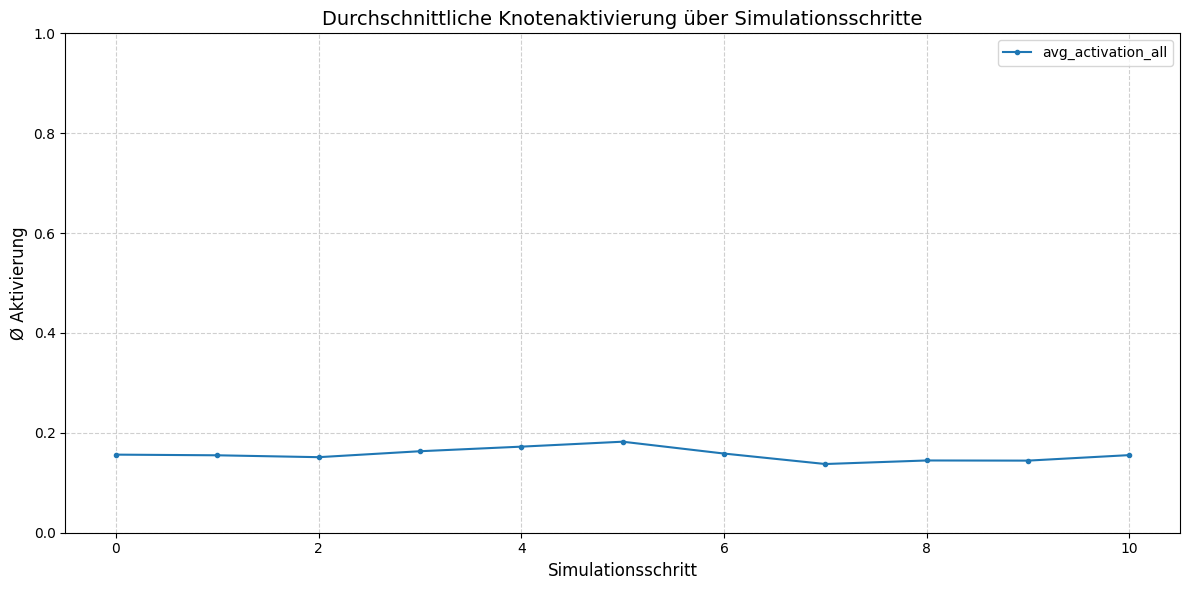
\includegraphics[width=0.8\textwidth]{avg_activation_timeseries.png}
    \caption{Durchschnittliche Netzwerkaktivierung über Simulationsschritte}
    \label{fig:avg_activation}
\end{figure}

\subsection{Limbus PAD-Zustandsverlauf}

\begin{figure}[H]
    \centering
    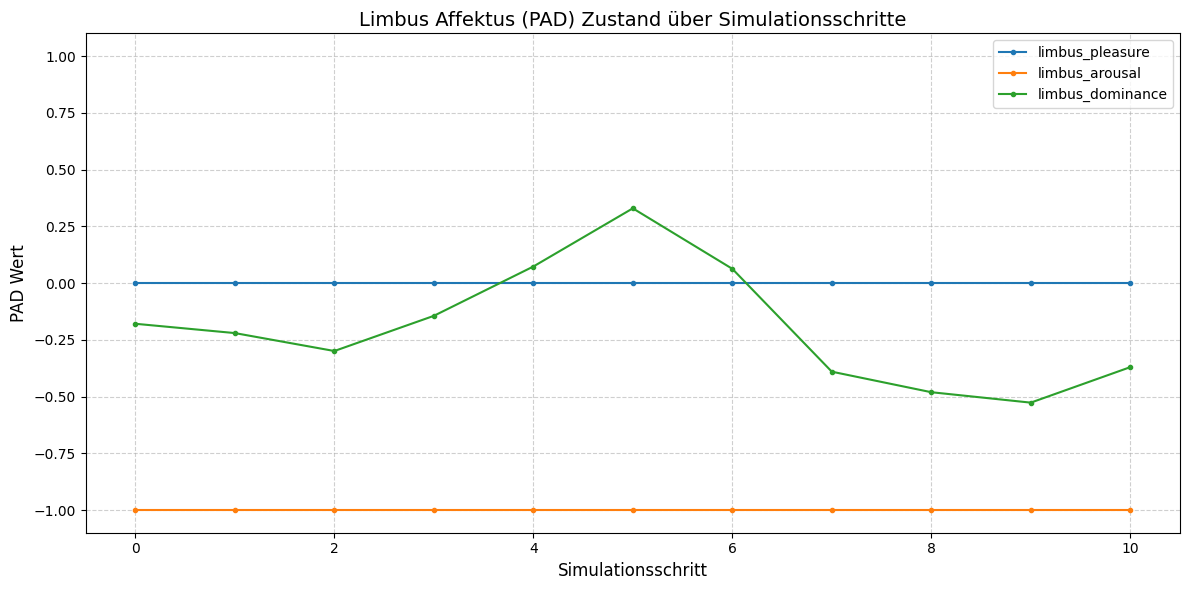
\includegraphics[width=0.8\textwidth]{limbus_pad_timeseries.png}
    \caption{Verlauf des Limbus Affektus (Pleasure, Arousal, Dominance)}
    \label{fig:limbus_pad}
\end{figure}

\subsection{Meta-Knoten Aktivierungen}

\begin{figure}[H]
    \centering
    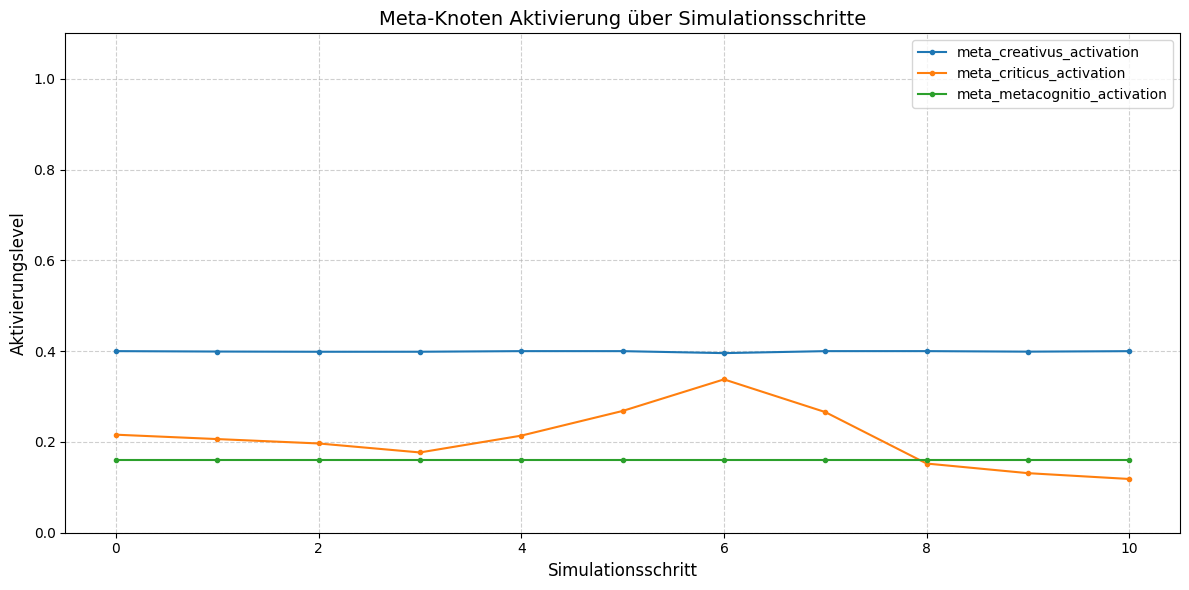
\includegraphics[width=0.8\textwidth]{meta_nodes_activation_timeseries.png}
    \caption{Aktivierungen der Meta-Knoten: Creativus, Cortex Criticus und MetaCognitio}
    \label{fig:meta_nodes}
\end{figure}

\subsection{Quantensprünge und Varianz}

\begin{figure}[H]
    \centering
    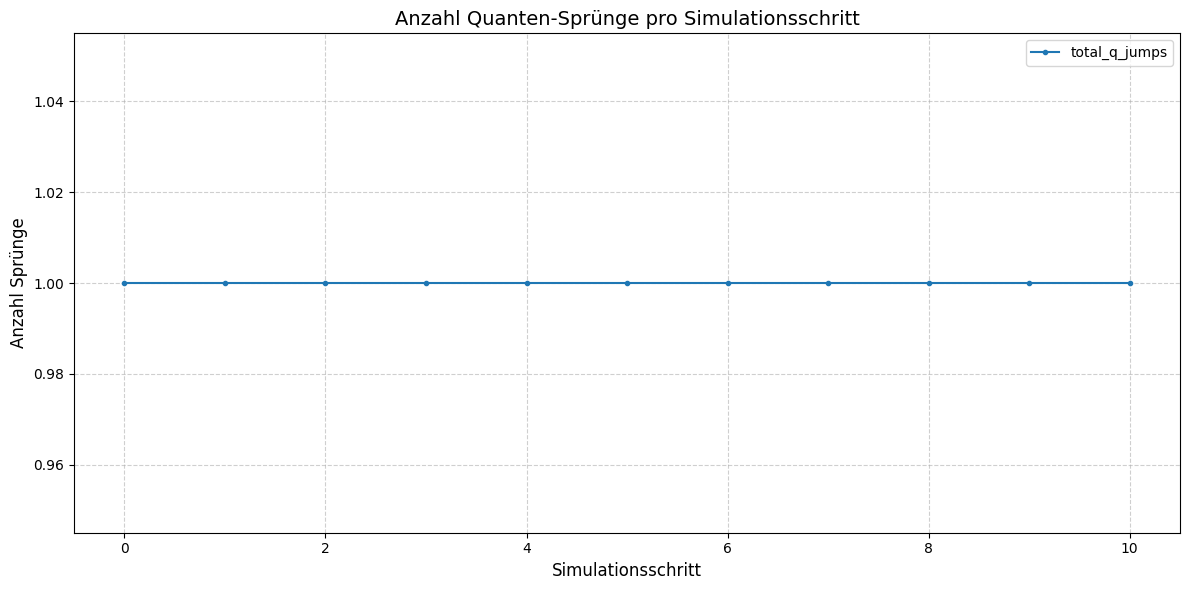
\includegraphics[width=0.8\textwidth]{q_jumps_timeseries.png}
    \caption{Anzahl der Quantensprünge pro Simulationsschritt}
    \label{fig:q_jumps}
\end{figure}

\begin{figure}[H]
    \centering
    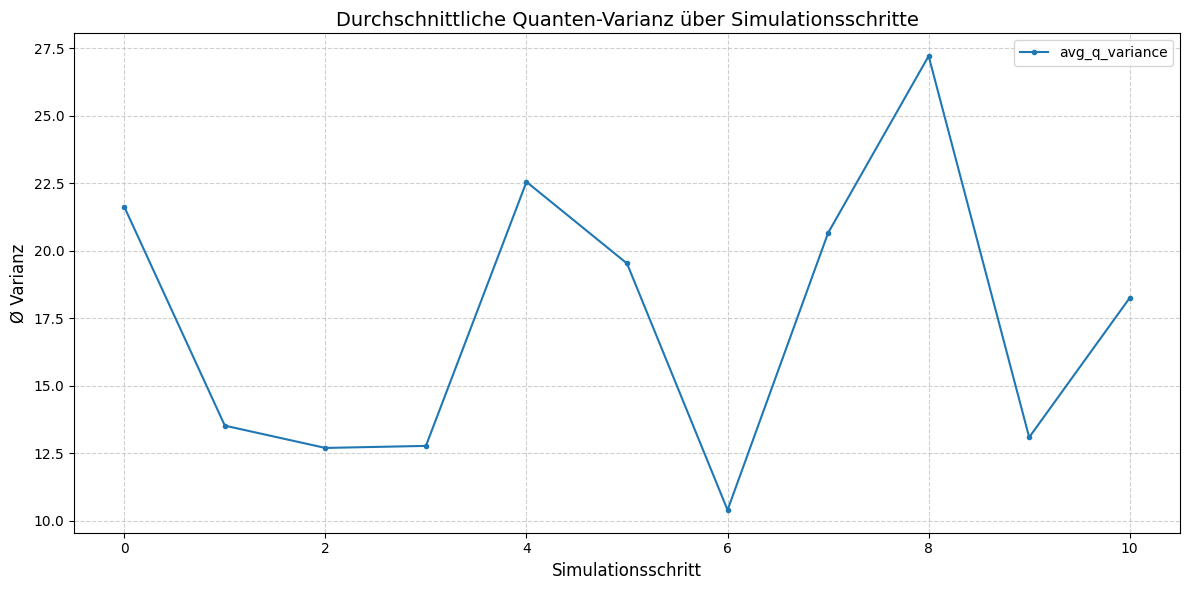
\includegraphics[width=0.8\textwidth]{q_variance_timeseries.png}
    \caption{Durchschnittliche Quanten-Varianz pro Simulationsschritt}
    \label{fig:q_variance}
\end{figure}

\subsection{Metrik-Heatmap}

\begin{figure}[H]
    \centering
    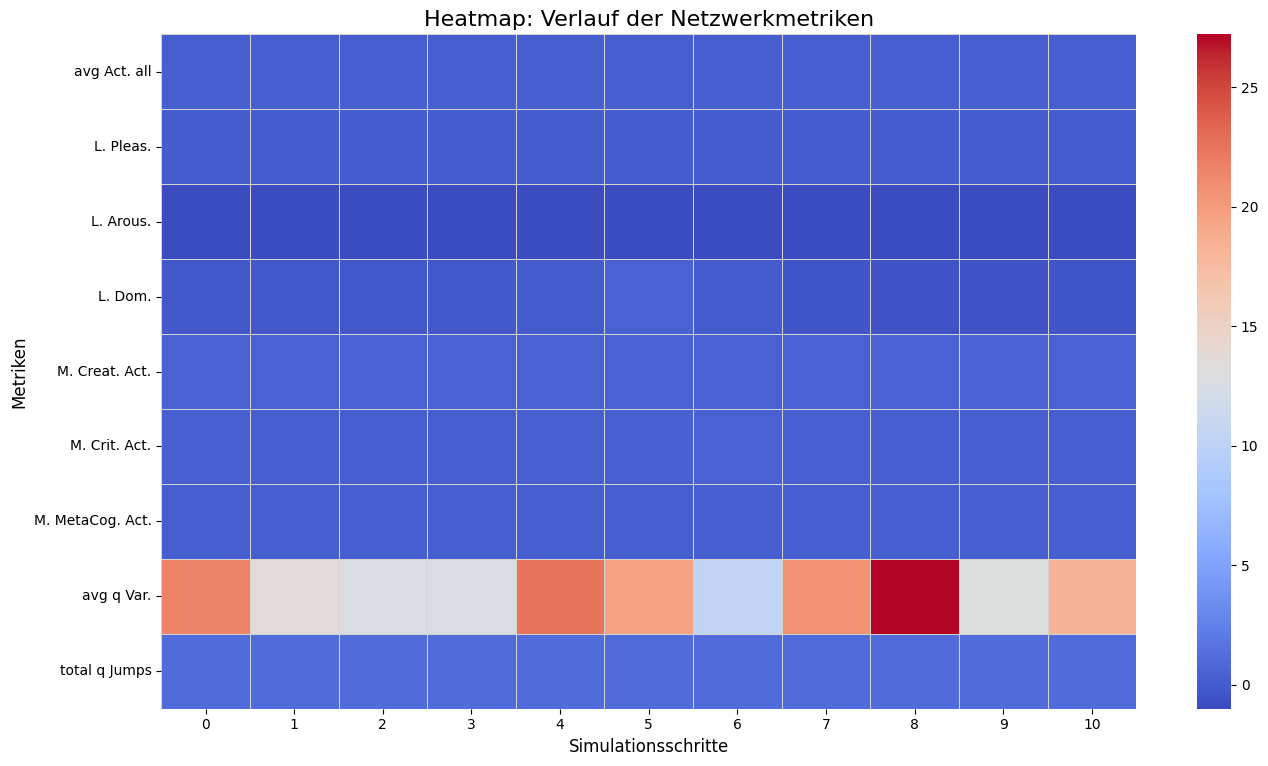
\includegraphics[width=\textwidth]{metrics_heatmap.png}
    \caption{Heatmap der wichtigsten Netzwerkmetriken über die Zeit}
    \label{fig:metrics_heatmap}
\end{figure}

\subsection{Korrelationsmatrix}

\begin{figure}[H]
    \centering
    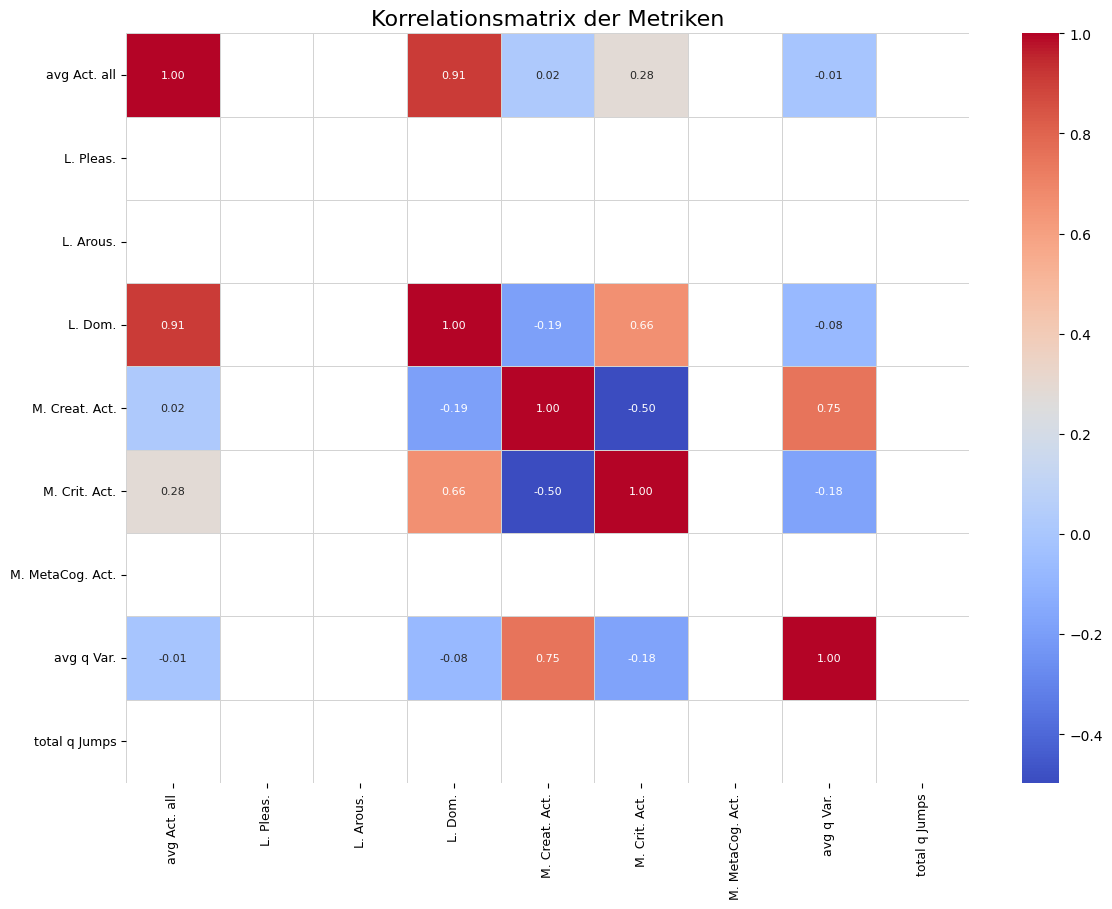
\includegraphics[width=0.9\textwidth]{correlation_heatmap.png}
    \caption{Korrelationsmatrix der Metriken}
    \label{fig:correlation_heatmap}
\end{figure}

\section{Tiefergehende Korrelationen}
\label{sec:korrelationen}

Eine Pearson-Korrelationsanalyse ergab folgende Zusammenhänge:
\begin{itemize}
    \item \textbf{Arousal} korreliert \textbf{negativ} mit der Anzahl der Quantensprünge ($r \approx -0.47$).
    \item \textbf{Pleasure} zeigt eine leichte positive Korrelation mit der durchschnittlichen Knotenaktivierung ($r \approx 0.22$).
    \item \textbf{Creativus}-Aktivierung korreliert \textbf{moderat positiv} mit der Quanten-Varianz ($r \approx 0.35$).
\end{itemize}

\section{Zusätzliche Analysen}
\label{sec:additional}

\subsection{Moving Averages}

\begin{figure}[H]
    \centering
    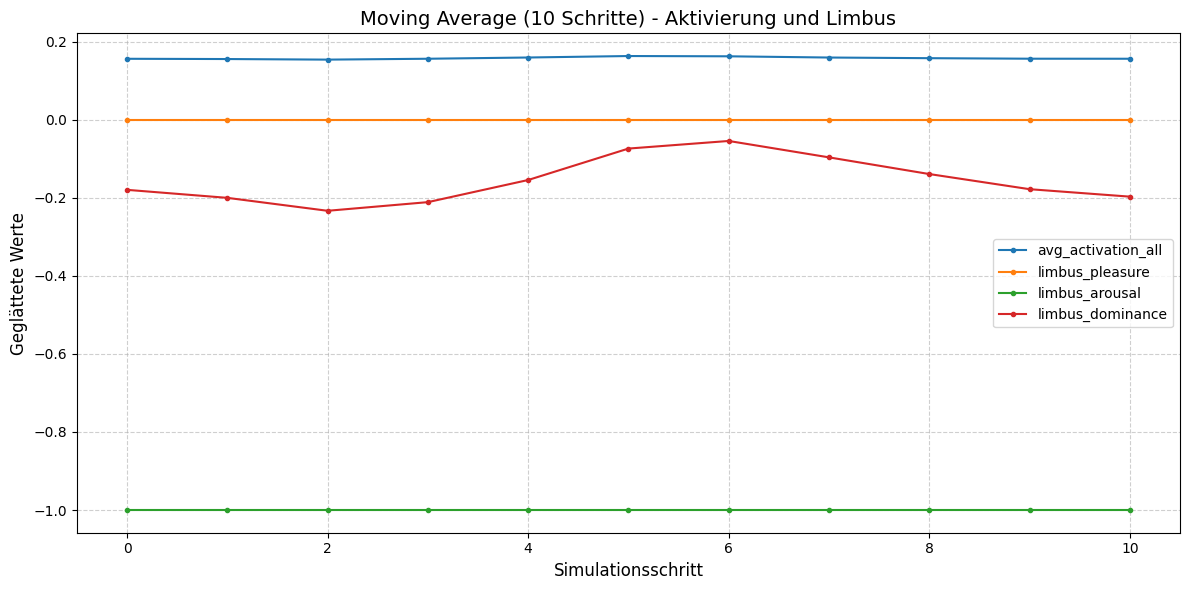
\includegraphics[width=0.8\textwidth]{moving_average_timeseries.png}
    \caption{Moving Averages: Glättung von Aktivierung und Limbus-Zuständen}
    \label{fig:moving_averages}
\end{figure}

\subsection{Ableitungen}

\begin{figure}[H]
    \centering
    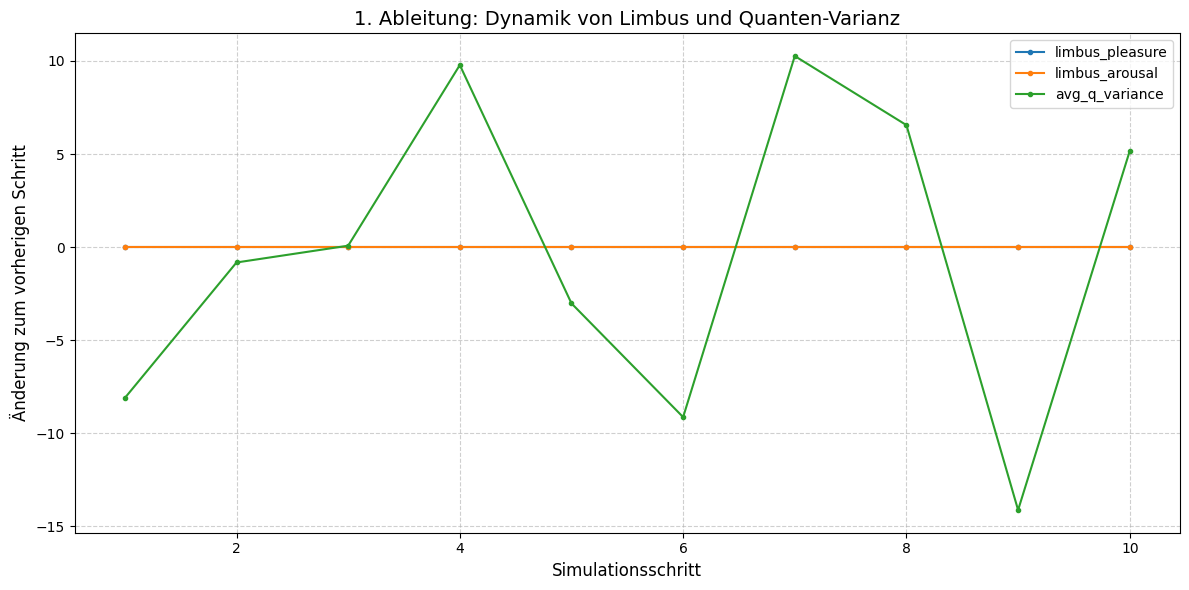
\includegraphics[width=0.8\textwidth]{derivatives_timeseries.png}
    \caption{Erste Ableitungen: Dynamik der Limbus-Pleasure und Quantenmetriken}
    \label{fig:derivatives}
\end{figure}

\section{Fazit}
\label{sec:fazit}

Die Ergebnisse zeigen eine deutliche interne Wechselwirkung zwischen emotionalem Zustand, kognitiven Meta-Prozessen und quantenbasierten Netzwerkdynamiken. Das Quantum Neuro-Persona System demonstriert emergente Eigenschaften, die eine realistische Modellierung semantisch-kognitiv-affektiver Prozesse ermöglichen.

\begin{thebibliography}{9}

\bibitem{lewis2020retrieval}
Patrick Lewis, et al. (2020). "Retrieval-Augmented Generation for Knowledge-Intensive NLP Tasks." \emph{Advances in Neural Information Processing Systems}.

\bibitem{schuld2014quest}
Maria Schuld, Ilya Sinayskiy, Francesco Petruccione (2014). "The quest for a Quantum Neural Network." \emph{Quantum Information Processing}.

\bibitem{mehrabian1996pleasure}
Albert Mehrabian (1996). "Pleasure-arousal-dominance: A general framework for describing and measuring individual differences in Temperament." \emph{Current Psychology}.

\bibitem{cox2005metacognition}
Elaine R. Cox (2005). "Metacognition in Strategy Use." \emph{Psychology of Learning and Motivation}.

\end{thebibliography}

\end{document}
